\documentclass[10.5pt,a4paper]{article}
\usepackage[margin=2.2cm]{geometry}
\usepackage{amsmath,amssymb,booktabs,graphicx,hyperref,enumitem,array}
\usepackage[T1]{fontenc}
\usepackage{lmodern}
\usepackage{microtype}
\hypersetup{colorlinks=true,linkcolor=black,citecolor=black,urlcolor=black}
\setlist{nosep,leftmargin=1.4em}
\setlength{\parskip}{3pt}

\title{\textbf{Trend Following with a Market-Neutral Core}}
\author{Jaakko Pakarinen \quad Eemil Ylä-Nikkilä \quad Erik Joonas Salumäe \quad Kristofer Vaiksaar\\[4pt]
\small Lynx Hackathon 2026, Stockholm}
\date{14 November 2026}

\begin{document}
\maketitle

\begin{abstract}
\noindent We present a futures portfolio built from two complementary books held at equal risk. The first, BOMBASTRAT, is a market-neutral combination of three established predictors: time-series momentum, an inflation-surprise signal for bonds and equities, and convergence of economically linked commodity pairs. The second, GOAT, holds stocks and bonds only while they trend, exits when a trend becomes stretched, and adds within-class momentum. The two books are driven by different mechanisms and have a return correlation of 0.36. Combined, the portfolio attains an adjusted Sharpe ratio of 1.16 net of costs over 1997--2016, with every sub-period at or above 1.00 and all twenty calendar years positive. Each component has an economic rationale, a closed-form definition and a falsification test, and performance is stable across neighbouring parameter values. Positions pass both look-ahead tests specified by the organisers.
\end{abstract}

\section{Introduction}
Trend following is the most robustly documented source of return in futures markets (Moskowitz, Ooi and Pedersen, 2012; Hurst, Ooi and Pedersen, 2017), but it has a well-known weakness: it earns little in markets that reverse or drift without direction. The objective of this work is a portfolio that keeps the long-run return of trend following while removing its dependence on any single market environment.

Our approach rests on three principles. Every component must have an economic mechanism that explains why it should work out of sample. Every component must be defined by an explicit formula with a small number of parameters fixed in advance. And every component must be falsifiable: it must stop working when its mechanism is removed. The result is a portfolio whose core takes no directional market risk, complemented by a trend-conditioned allocation to stocks and bonds.

\section{Data and evaluation}
The universe consists of 27 futures: bonds and equity indices for five economies, four currency pairs and thirteen commodities, observed daily from 1995 to 2016, together with CPI and GDP for each economy.

Let $P_{t,i}$ be the price of asset $i$ on day $t$ and $\Delta P_{t,i}=P_{t,i}-P_{t-1,i}$. A position $x_{t,i}$ determined with information up to day $t$ earns $x_{t,i}(P_{t+2,i}-P_{t+1,i})$ and incurs a cost of $c\,\sigma_{t,i}\,|x_{t,i}-x_{t-1,i}|$, $c=0.02$. Performance is measured by the adjusted Sharpe ratio
\begin{equation}
\mathrm{ASR}=\mathrm{SR}\left(1+\frac{S}{6}\,\mathrm{SR}-\frac{K}{24}\,\mathrm{SR}^2\right),
\end{equation}
where SR is the annualised Sharpe ratio of daily net P\&L, $S$ its skewness and $K$ its excess kurtosis. Since ASR does not depend on the scale of positions, the design goal is the stability of risk-adjusted returns, not leverage. All figures are computed with the organisers' \texttt{evaluation.py} from 22 May 1997, the first date on which every component holds positions.

\section{Research path}
The portfolio was built in stages. At each stage we asked what the existing model failed to capture and which mechanism could address it.

\begin{enumerate}
\item \textbf{Establishing the effects.} Before any backtest we measured which relationships exist in the data. Trend is present in every asset class. Inflation predicts bond and equity returns with the same sign in all five economies. Single-asset reversion is absent. The 27 assets behave like roughly 13 independent ones, and three commodity pairs move together more than 80\% of the time.
\item \textbf{Trend as the foundation.} Time-series momentum alone scores 0.82, against 0.32 for the organisers' reference strategy. It is strong in 1997--2002 (1.57) but fades to 0.40 in 2009--2016.
\item \textbf{Inflation as a diversifier.} Trend is a statement about prices; inflation is a statement about the economy. The inflation signal is uncorrelated with trend ($\rho=-0.06$) and is strongest in 2002--2009, when trend is weakest. Together they score 1.01.
\item \textbf{Twins for reversion.} Since single prices do not revert, reversion needs an anchor. Two forms of the same good provide one: their spread is held in place by substitution. Adding the twin pairs raises the score to 1.11 and lifts 2009--2016 from 0.48 to 0.63. This is BOMBASTRAT.
\item \textbf{Addressing the remaining weakness.} BOMBASTRAT's weakest period, 2009--2016, was a period of steadily rising stock and bond prices with few reversals. GOAT was developed in parallel for exactly this environment: it is long stocks and bonds only while their trend is intact and steps aside when the trend becomes stretched. It scores 1.00 in 2009--2016 and 0.84 in 1997--2002, the mirror image of BOMBASTRAT.
\item \textbf{One portfolio.} Held at equal risk, the two books lift the weakest sub-period from 0.63 to 1.00 and the full-period score to 1.16.
\end{enumerate}

\section{The core: BOMBASTRAT}
All statistics are trailing and use information up to day $t$ only. Volatility is $\sigma_{t,i}=0.7\,v_{t,i}+0.3\,\bar v^{(500)}_{t,i}$, with $v_{t,i}$ the exponentially weighted root-mean-square of $\Delta P_{t,i}$ (span 35) and $\bar v^{(500)}$ its 500-day mean. Forecasts are bounded with $\tanh(\cdot)$, which is linear near zero and saturates at $\pm1$, limiting the influence of extreme readings on the tails of the P\&L.

\subsection{Time-series momentum}
\textit{Mechanism.} Investors under-react to new information and adjust positions gradually, so price moves persist over horizons of months.

\textit{Definition.} With $\tilde P$ the price series with daily changes winsorised at $5\sigma$ and $\mathrm{EMA}_n$ an exponential moving average of span $n$,
\begin{equation}
r^{(n,m)}_{t}=\frac{\mathrm{EMA}_n(\tilde P)_t-\mathrm{EMA}_m(\tilde P)_t}{\sigma_t},\qquad
M_t=\frac{1}{\sigma_t\sqrt{250}}\sum_{s=t-249}^{t}\Delta\tilde P_s .
\end{equation}
Each is divided by its expanding mean absolute value and capped at $\pm2$ (denoted by a hat), and
\begin{equation}
f^{\mathrm{TR}}_t=\tfrac12\Bigl[\tfrac12\bigl(\hat r^{(32,128)}_t+\hat r^{(64,256)}_t\bigr)+\hat M_t\Bigr],
\end{equation}
applied to all 27 assets. The crossovers capture trends of two to twelve months; the 12-month return is the canonical momentum measure.

\subsection{Inflation surprise}
\textit{Mechanism.} Inflation above its recent norm raises expected policy rates, which lowers bond prices directly and equity valuations through the discount rate.

\textit{Definition.} For each economy, with $C_t$ the latest available CPI and horizon $k=60$ days for bonds and $k=120$ for equities,
\begin{equation}
g_t=\ln C_t-\ln C_{t-k},\qquad
z_t=\frac{g_t-\bar g^{(750)}_t}{\operatorname{sd}^{(750)}_t\!\left(g-\bar g^{(750)}\right)},\qquad
f^{\mathrm{INF}}_t=-\tanh(z_t).
\end{equation}
Inflation is measured against its own trailing three-year norm. The signal is applied to the five bond and five equity futures.

\subsection{Twin-pair convergence}
\textit{Mechanism.} The relative price of two forms of the same good is anchored by substitution and arbitrage: when one becomes cheap relative to the other, demand shifts and the spread closes (Gatev, Goetzmann and Rouwenhorst, 2006).

\textit{Definition.} Assets $a,b$ are twins on day $t$ if the correlation of their five-day price changes over all data up to $t$ (at least 250 days) exceeds 0.8; three commodity pairs qualify. With log spread $s_t=\ln P_{t,a}-\ln P_{t,b}$,
\begin{equation}
z_t=\frac{s_t-\bar s^{(250)}_t}{\operatorname{sd}^{(250)}_t(s)},\qquad
f^{\mathrm{TW}}_{t,a}=-\tanh(z_t/2),\qquad f^{\mathrm{TW}}_{t,b}=+\tanh(z_t/2),
\end{equation}
so the book sells the expensive leg and buys the cheap one, with no net exposure to the pair.

\subsection{Construction}
Each signal $k$ is scaled by $s^k_t$, the 250-day volatility of its own stand-alone P\&L, so the three contribute equal risk: $F_t=\sum_k f^k_t/s^k_t$. Positions are $\hat x_{t,i}=F_{t,i}/\sigma_{t,i}$, giving equal risk per asset, and are scaled to constant ex-ante volatility, $x^*_t=\hat x_t/\sqrt{\hat x_t^{\top}\Sigma_t\hat x_t}$, with $\Sigma_t$ the 250-day covariance of price changes. Execution is smoothed, $x_t=0.3\,x^*_t+0.7\,x_{t-1}$, to balance signal decay against costs.

\section{The trend overlay: GOAT}
\subsection{Engine 1: trend-conditioned exposure to stocks and bonds}
\textit{Mechanism.} Stocks and bonds carry long-run risk premia, but holding them through sustained declines is costly. Conditioning the position on trend keeps the premium while stepping aside in drawdowns. Trends that become extended relative to volatility are prone to sharp reversals, so a trailing stop is activated only once a trend is stretched.

\textit{Definition.} For each of the ten stocks and bonds, with $\sigma^{(100)}_t$ the 100-day root-mean-square of price changes,
\begin{equation}
d_t=\frac{\mathrm{EMA}_{10}(P)_t-\mathrm{EMA}_{100}(P)_t}{\sigma^{(100)}_t},\qquad
e_t=\begin{cases}1 & \text{if } d_t>0 \text{ and the stop is not triggered},\\ 0 & \text{otherwise.}\end{cases}
\end{equation}
When $d_t\ge 7$ a trailing stop is armed. After three consecutive rising closes the stop is set at the lowest of them and only ratchets upwards. A close below the stop sets the position to zero until $d_t$ falls back below 7 or a new crossover occurs. The engine is long or flat, never short.

\subsection{Engine 2: momentum within asset classes}
\textit{Mechanism.} Within a class, assets with the strongest twelve-month performance tend to continue to outperform the weakest (Asness, Moskowitz and Pedersen, 2013).

\textit{Definition.} With $\rho_{t,i}\in\{1,\dots,n_c\}$ the rank of asset $i$'s 252-day return within its class $c$, $q_{t,i}=2(\rho_{t,i}/n_c-\tfrac12)$.

\subsection{Construction}
The engines are combined as $u_t=0.6\,e_t/\sigma^{(100)}_t+0.4\,q_t/\sigma^{(100)}_t$, smoothed with $x_t=0.25\,u_t+0.75\,x_{t-1}$, and a position is changed only when the relative change exceeds 10\%, which suppresses small trades.

\section{The combined portfolio}
Both books are scaled to the same constant ex-ante volatility using the 250-day covariance of price changes, and the final position is their average,
\begin{equation}
x^{\mathrm{final}}_t=\tfrac12\,x^{\mathrm{BOMBA}}_t+\tfrac12\,x^{\mathrm{GOAT}}_t .
\end{equation}
Equal weighting is the natural prior for two books of equal risk, and we did not optimise it: any weight on GOAT between 20\% and 67\% gives a full-period score between 1.13 and 1.16 (Figure~\ref{fig:weights}).

\section{Results}
\begin{table}[h]
\centering\small
\setlength{\tabcolsep}{4.5pt}\begin{tabular}{lccccccc}
\toprule
 & ASR & 1997--02 & 2002--09 & 2009--16 & Worst 3y & Positive yrs & Net exp. \\
\midrule
\textbf{Combined} & \textbf{1.16} & \textbf{1.00} & \textbf{1.27} & \textbf{1.00} & \textbf{0.36} & \textbf{20 of 20} & 0.28 \\
BOMBASTRAT & 1.11 & 1.34 & 1.27 & 0.63 & $-0.10$ & 18 of 20 & 0.00 \\
GOAT & 0.95 & 0.84 & 0.97 & 1.00 & 0.38 & 20 of 20 & 0.62 \\
Momentum only & 0.82 & 1.57 & 0.73 & 0.40 & & & 0.08 \\
Reference (50-day sign) & 0.32 & $-0.07$ & 0.55 & 0.28 & & & 0.02 \\
\bottomrule
\end{tabular}
\caption{Adjusted Sharpe ratio net of costs with two-day lag. GOAT is shown at constant risk, as it enters the portfolio. Net exposure is the evaluator's position bias (0 = balanced, 1 = always long).}
\end{table}

\begin{figure}[h]
\centering
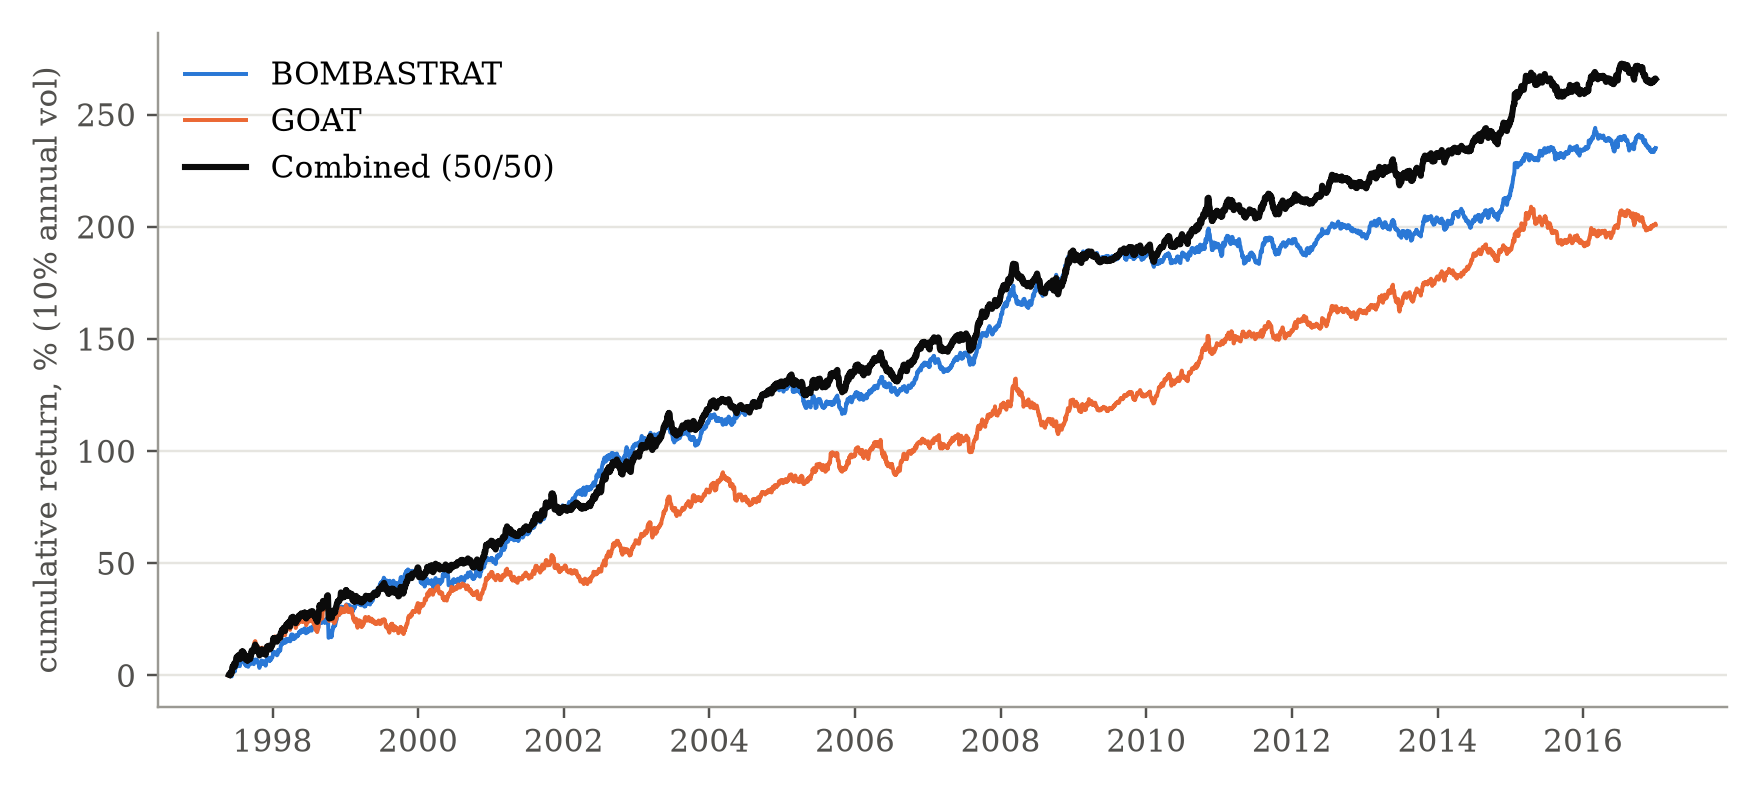
\includegraphics[width=0.84\linewidth]{fig_equity.png}
\caption{Cumulative net return, each book scaled to 10\% annual volatility.}
\end{figure}

The combined portfolio has a Sharpe ratio of 1.36 net and 1.43 before costs, skewness $-0.15$, kurtosis 4.51 and an average holding period of 39 days. One additional day of execution lag changes the Sharpe ratio from 1.36 to 1.35.

\textbf{The combination raises the floor, not the peak.} The full-period score improves modestly, from 1.11 to 1.16, but the weakest sub-period improves from 0.63 to 1.00, the worst three-year window from $-0.10$ to 0.36, and the number of losing years from two to none. The two books succeed in different environments: BOMBASTRAT in markets with large trends and inflation shocks, GOAT in steadily rising markets.

\begin{figure}[h]
\centering
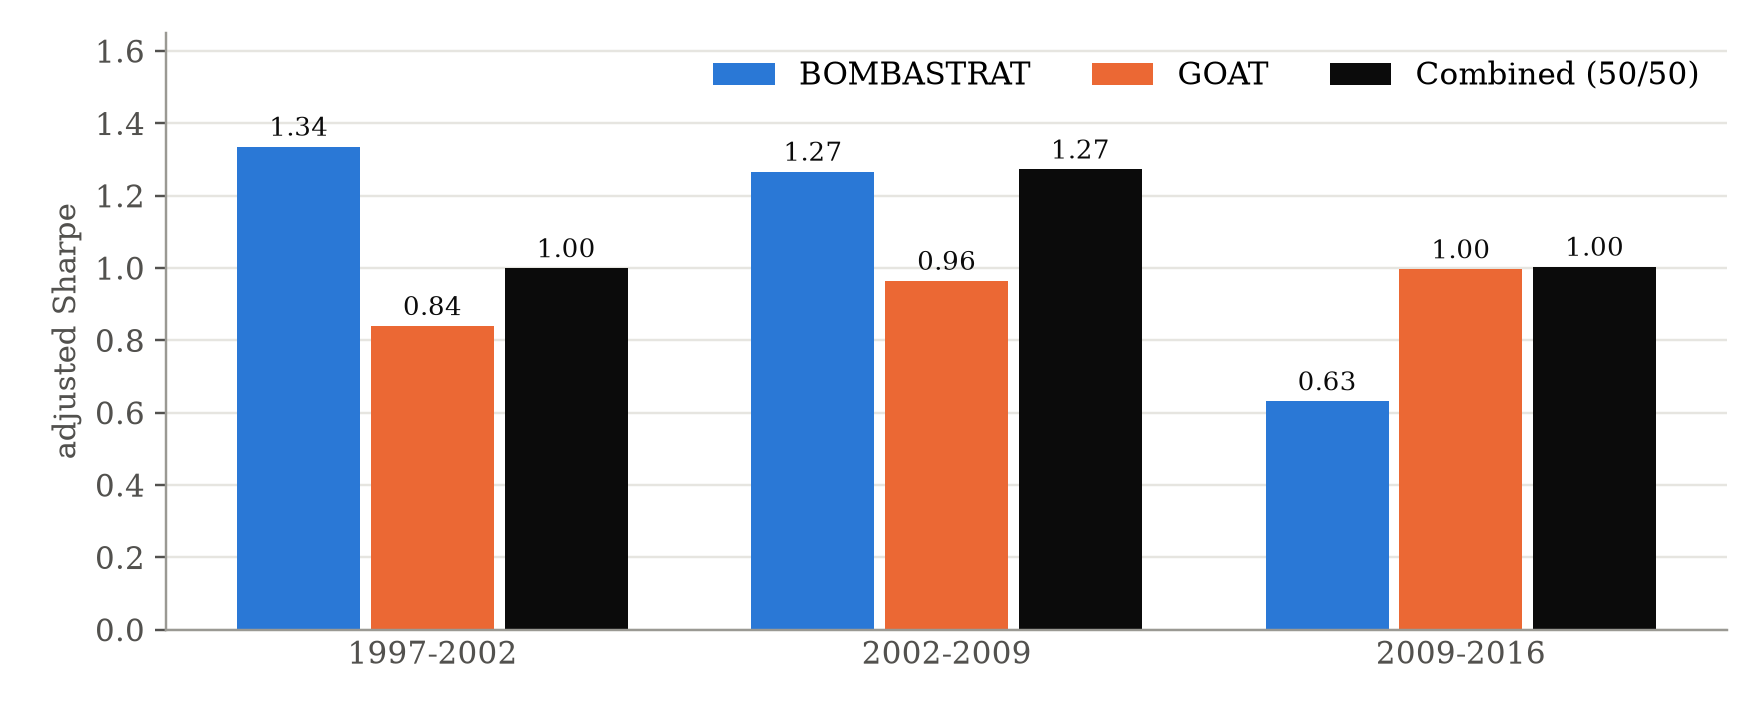
\includegraphics[width=0.84\linewidth]{fig_eras.png}
\caption{Adjusted Sharpe ratio by sub-period.}
\end{figure}

\textbf{Market exposure.} The core is market-neutral: BOMBASTRAT's net exposure is 0.00 and its return correlation with a passive stock and bond portfolio is 0.16. GOAT contributes a deliberate long exposure, held only while trends are intact. The combined net exposure is 0.28 and the correlation with the passive portfolio 0.53, against 0.70 for GOAT alone. In the two years in which the passive portfolio lost money, 2001 and 2008, the market-neutral core scored 2.14 and 1.20.

\section{Robustness}
\subsection{Falsification tests}
\begin{table}[h]
\centering\small
\begin{tabular}{p{6.6cm}p{3.4cm}p{4.8cm}}
\toprule
Test & Result & Interpretation \\
\midrule
Inflation signal with CPI lagged one year & $-0.14$ (vs 0.72) & predictive content lies in timely data \\
Inflation signal, each economy separately & positive in 5 of 5 & consistent across economies \\
Twin rule on 40 random non-twin pairs & mean $-0.06$, max 0.21 & requires a genuine economic link \\
Momentum with every price path inverted & 0.87 (vs 0.82) & independent of market direction \\
Leak test: shorter history & identical positions & no look-ahead \\
Leak test: future data replaced & identical positions & no look-ahead \\
\bottomrule
\end{tabular}
\caption{Placebo results refer to each signal on its own. Leak tests are the two methods in the organisers' instructions, applied to the final portfolio with prices and macro data.}
\end{table}

\subsection{Parameter sensitivity}
Every parameter was set in advance at a round value. Varying them shows broad plateaus rather than isolated optima.

\begin{figure}[h]
\centering
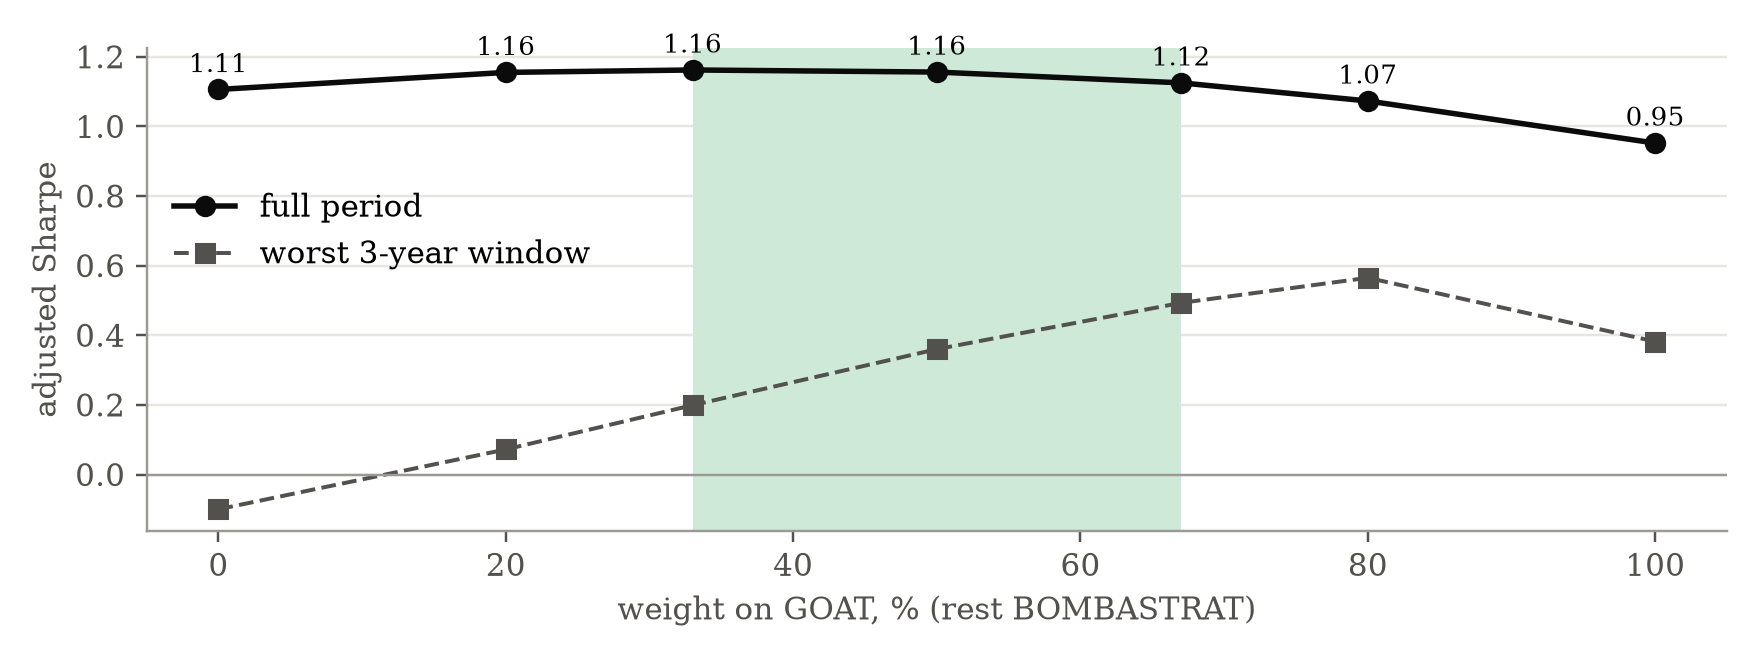
\includegraphics[width=0.78\linewidth]{fig_weights.png}
\caption{Weight on GOAT. The shaded region (33--67\%) scores 1.13 to 1.16. The worst three-year window rises from $-0.10$ for BOMBASTRAT alone to 0.36 at equal weights.}\label{fig:weights}
\end{figure}

\begin{figure}[h]
\centering
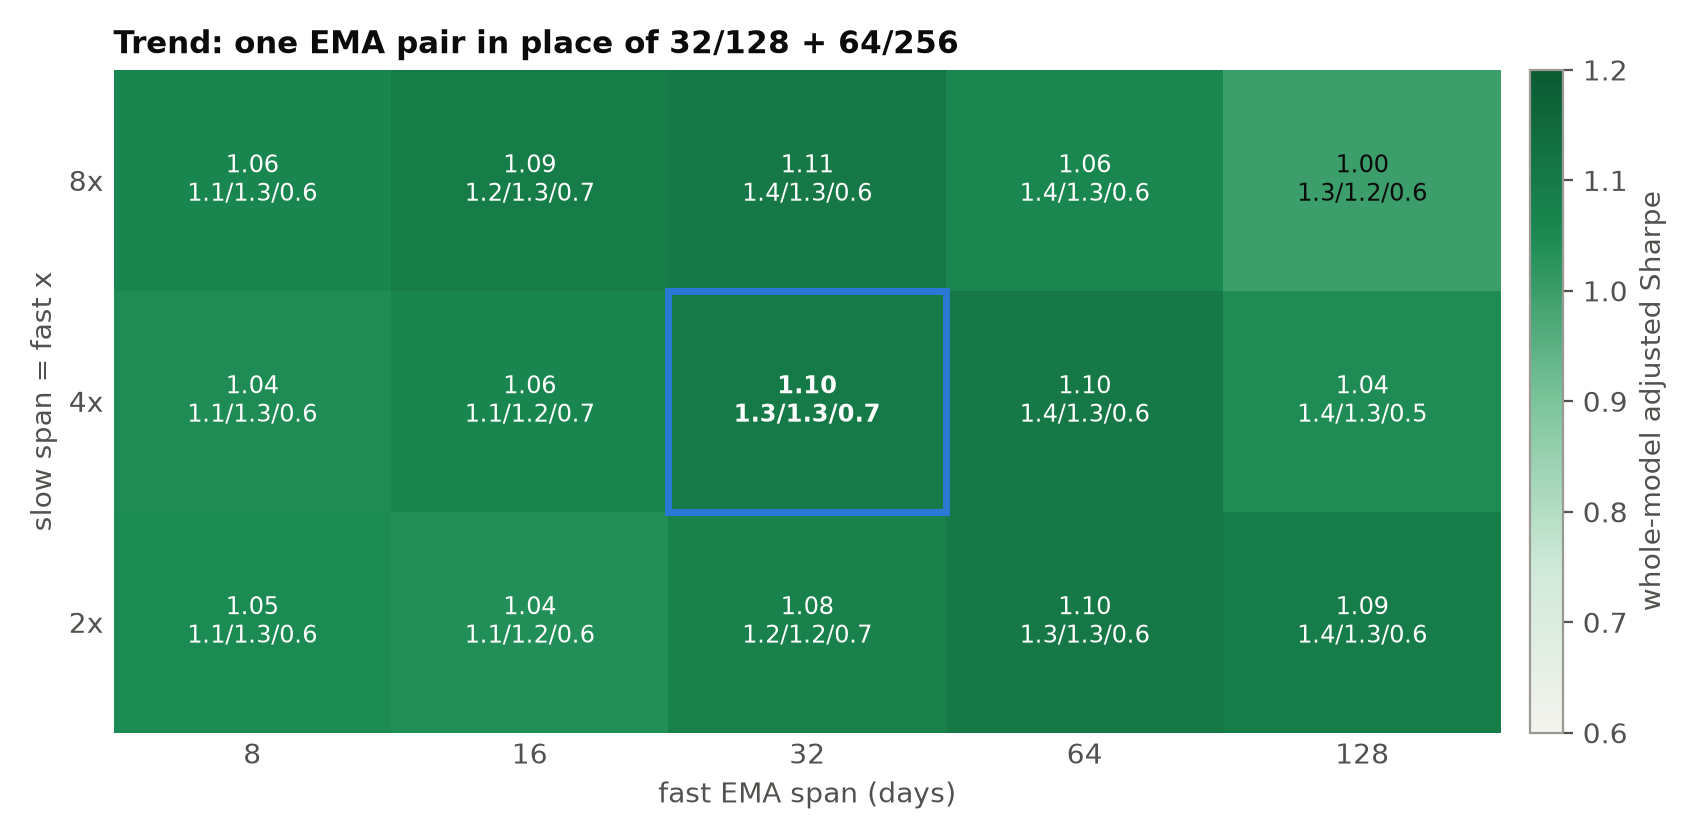
\includegraphics[width=0.75\linewidth]{fig_trend.png}
\caption{BOMBASTRAT with one trend crossover in place of 32/128 and 64/256. All fifteen specifications score between 1.00 and 1.11. Small figures give the three sub-periods.}
\end{figure}

\begin{figure}[h]
\centering
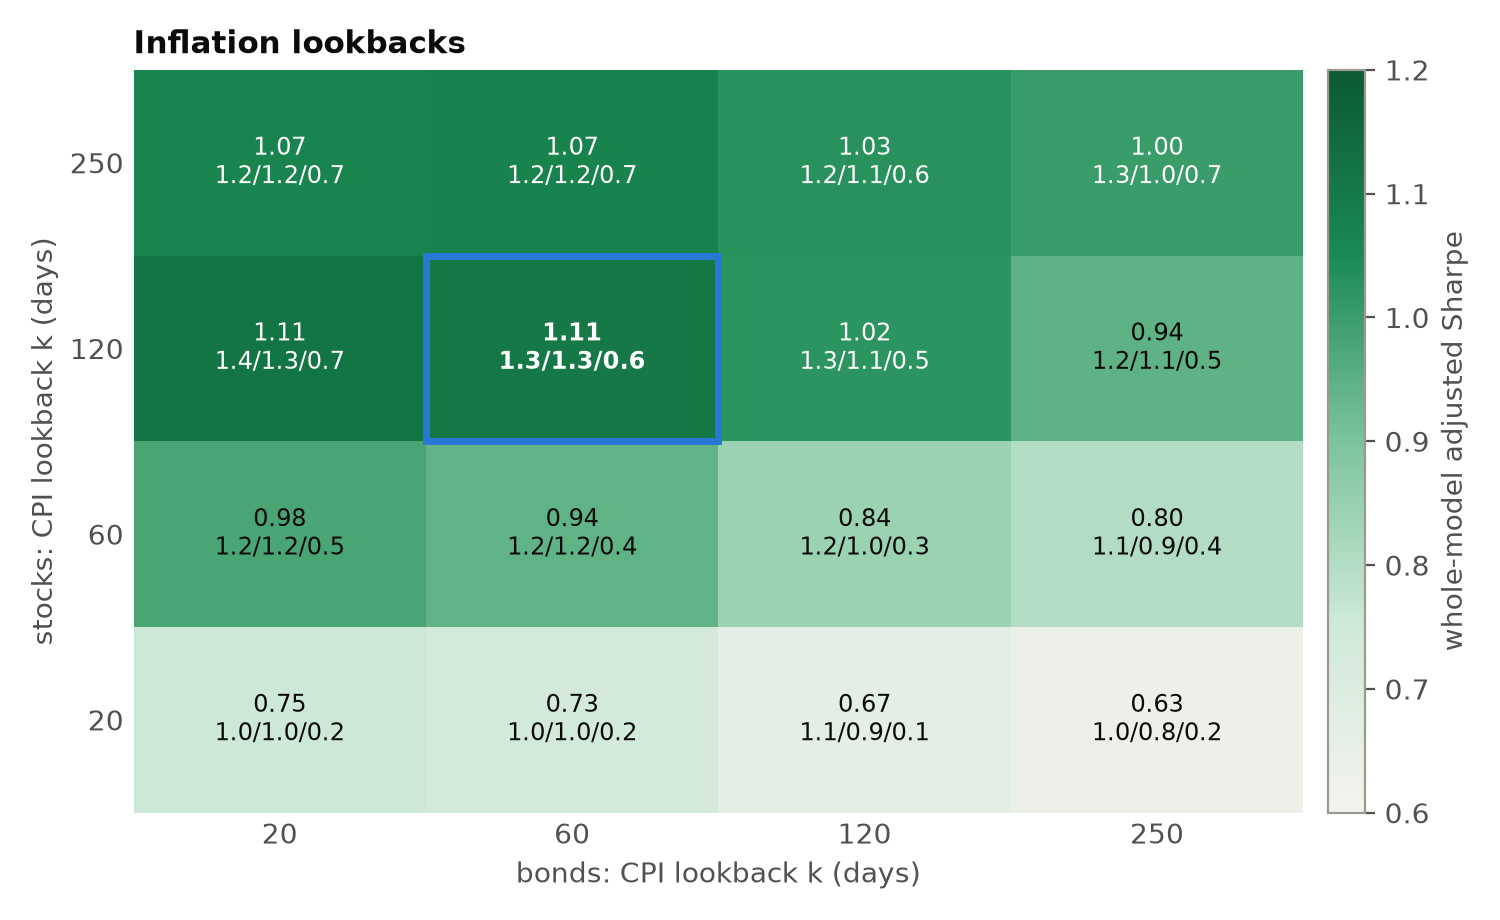
\includegraphics[width=0.49\linewidth]{fig_inflation.png}\hfill
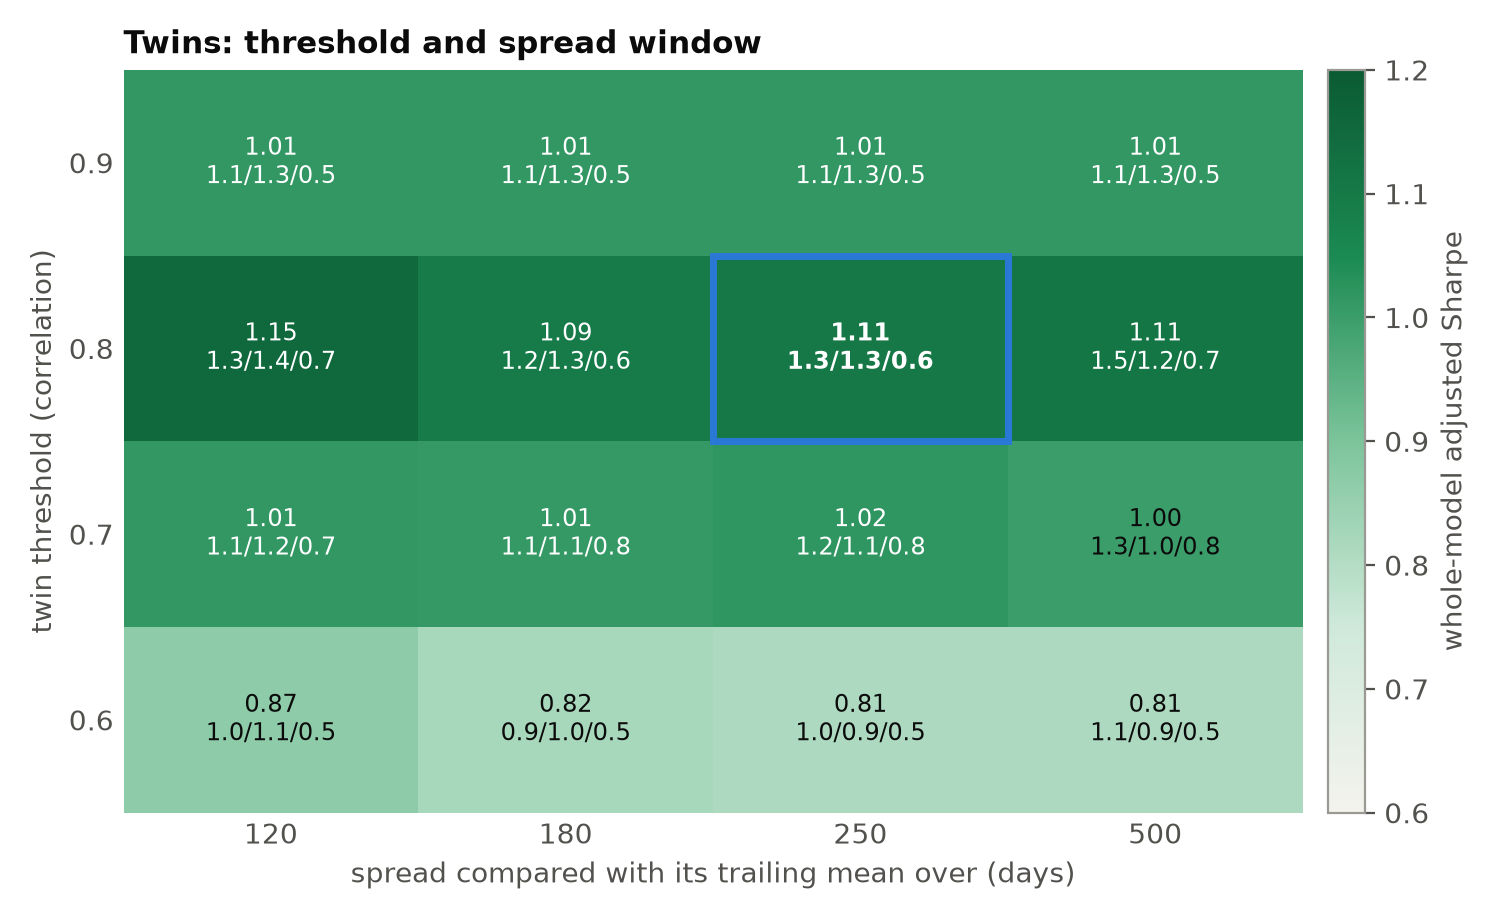
\includegraphics[width=0.49\linewidth]{fig_twins.png}
\caption{BOMBASTRAT under alternative inflation horizons (left) and twin parameters (right). Any equity horizon of 120--250 days yields 1.00--1.11; only a 20-day horizon degrades, consistent with equities pricing persistent rather than transitory inflation. Twin thresholds of 0.7--0.9 yield 1.00--1.15; at 0.6 unrelated pairs enter and the score falls, replicating the placebo.}
\end{figure}

\begin{table}[h]
\centering\small
\begin{tabular}{lcccc}
\toprule
GOAT setting & Full & 1997--2002 & 2002--2009 & 2009--2016 \\
\midrule
As used & 1.02 & 0.88 & 1.12 & 1.01 \\
Stop threshold 6 / 8 / 10 & 1.00 / 1.01 / 0.98 & & & \\
Engine weights 50/50 / 70/30 & 0.98 / 1.02 & & & \\
Smoothing 10\% / none & 0.97 / 0.98 & & & \\
Band off / 20\% & 1.01 / 0.99 & & & \\
Momentum lookback 190 / 310 days & 0.88 / 0.96 & & & \\
\bottomrule
\end{tabular}
\caption{GOAT sensitivity, one setting at a time (GOAT alone, before constant-risk scaling). As used: stop at 7, engines 60/40, smoothing 25\%, band 10\%, momentum 252 days.}
\end{table}

\section{Limitations}
\begin{enumerate}
\item The combined portfolio carries a net long exposure of 0.28. Part of GOAT's return is the passive premium on stocks and bonds, which a prolonged joint decline in both would remove; the market-neutral core is designed to carry the portfolio in that case.
\item The twin component rests on three commodity pairs, of which one contributes most.
\item All sub-periods were observed during development. Parameters were set in advance and the weight between the books was not optimised, but the out-of-sample period is the only clean test.
\end{enumerate}

\section{Conclusion}
The portfolio combines a market-neutral core of three textbook forecasts with a trend-conditioned allocation to stocks and bonds. Each component has a clear mechanism, an explicit definition and a falsification test, and the result is insensitive to its parameters. The two books succeed in different environments, and together they deliver an adjusted Sharpe ratio of 1.16 with no sub-period below 1.00 and no losing year.

\section*{References}
{\small
\begin{itemize}[leftmargin=0pt,label={},itemsep=2pt]
\item Asness, C.S., Moskowitz, T.J., Pedersen, L.H. (2013). Value and momentum everywhere. \textit{Journal of Finance} 68(3), 929--985.
\item Gatev, E., Goetzmann, W.N., Rouwenhorst, K.G. (2006). Pairs trading: performance of a relative-value arbitrage rule. \textit{Review of Financial Studies} 19(3), 797--827.
\item Hurst, B., Ooi, Y.H., Pedersen, L.H. (2017). A century of evidence on trend-following investing. \textit{Journal of Portfolio Management} 44(1), 15--29.
\item Moskowitz, T.J., Ooi, Y.H., Pedersen, L.H. (2012). Time series momentum. \textit{Journal of Financial Economics} 104(2), 228--250.
\end{itemize}

\textbf{Code.}
\begin{itemize}[leftmargin=1.2em,itemsep=1pt]
\item \texttt{SUBMISSION/model.py}: the complete model
\item \texttt{SUBMISSION/check.py}: leak tests and key figures
\item \texttt{SUBMISSION/whitepaper/make\_figures.py}: every number and figure in this paper
\end{itemize}}
\end{document}
